\documentclass[12pt]{article}

\usepackage{array}
\usepackage{adjustbox}
\usepackage{amsfonts}
\usepackage{amsmath}
\usepackage{amsthm}
\usepackage{amssymb}
\usepackage{dirtytalk}
\usepackage[a4paper, total={7in, 9in}]{geometry}
\usepackage{forest}
\usepackage{geometry}
\usepackage{multirow}
\usepackage{skak}
\usepackage{tikz}
\usepackage{titling}
\usepackage{wrapfig}
\usepackage{xcolor}

\usetikzlibrary{patterns}

\def\multichoose#1#2{\ensuremath{\left(\kern-.3em\left(\genfrac{}{}{0pt}{}{#1}{#2}\right)\kern-.3em\right)}}

\usetikzlibrary{decorations.pathreplacing}
\usetikzlibrary{patterns}

\pgfdeclarepatternformonly{bigger north west lines}{\pgfqpoint{-2pt}{-2pt}}{\pgfqpoint{8pt}{8pt}}{\pgfqpoint{6pt}{6pt}}%
{
  \pgfsetlinewidth{1pt}
  \pgfpathmoveto{\pgfqpoint{0pt}{6pt}}
  \pgfpathlineto{\pgfqpoint{6.2pt}{-0.2pt}}
  \pgfusepath{stroke}
}

\newcommand*{\Scale}[2][4]{\scalebox{#1}{$#2$}}
\newcommand*{\SetHeight}[2]{\resizebox{!}{#1}{$#2$}}

\begin{document}
\pagenumbering{gobble}

\title{Math 142 Study Guide}
\date{2016-10-06}
\author{David Alves}

\begin{center}
\large \thetitle \\
by \theauthor \\
\end{center}
\tableofcontents

\section{Notation \& Basics}
\newcommand{\termtable}[1]{
    \def\arraystretch{1.75}
    \begin{tabular}{ r|p{28em} }
    #1
    \end{tabular}
}
\newcommand{\term}[1]{\textbf{#1}&}

\termtable{
    \term{set} A collection of elements where the order doesn't matter and every element is distinct (You can't have two elements that are equal to each other)\\
    \term{list or $k-$tuple} A collection of elements $(a_1, a_2, \ldots, a_k)$ where the order matters and duplicates are allowed. For example $(1, 2)$ is different from $(2,1)$ and $(1,1)$ is a valid list.\\
    \term{$a \in A$} $a$ is an element of the set $A$\\
    \term{$a \notin A$} $a$ is \textbf{not} an element of the set $A$\\
    \term{$|S|$} The number of elements in a set $S$ (\emph{cardinality} of $S$)\\
    \term{$A \cap B$} The \emph{intersection} of $A$ and $B$, namely the set of elements that are in both $A$ and $B$\\
    \term{$A \cup B$} The \emph{union} of $A$ and $B$, namely the set of elements that are either in $A$, in $B$, or in both\\
    \term{$A \subset B$} $A$ is a \emph{subset} of $B$, meaning $A$ contains only elements that are in $B$. (Note for this class $A$ and $B$ can be equal, we are not using \say{proper subset})\\
    \term{$A \times B$} The \emph{cartesian product} of sets $A$ and $B$, namely the set of every possible list $(a, b)$ where $a \in A$ and $b \in B$. Example: $A=\{1,2\}, B=\{3,4\},A \times B = \{(1, 3), (1, 4), (2, 3), (2, 4)\}$\\
    \term{$\emptyset$ or $\{\}$} The empty set, the set with no elements\\
    \term{disjoint} Sets $A$ and $B$ are disjoint if they have no elements in common, meaning $A \cap B = \emptyset$\\
    \term{$\binom{n}{k}$} Number of subsets of size $k$ in a set of $n$ items, $\frac{n!}{k!(n-k)!}$\\

    \term{domain} The set of values that can go into a function. By definition a function can be applied to every element of the domain\\
    \term{codomain} That set of values that can come out of a function\\
    \term{injective} Every element in the codomain is hit at \textbf{most} once\\
    \term{surjective} Every element in the codomain is hit at \textbf{least} once\\
    \term{bijective} Every element of the codomain is hit \textbf{exactly} once (both injective and surjective)\\
    \term{$f : A \rightarrow B$} A function $f$ with domain $A$ and codomain $B$\\
    \term{$[n]$} The set of integers $\{1, 2, \ldots, n-1, n\}$\\
}
\pagebreak
\section{Basic Principles}
\subsubsection{Sum Principle}
\[
    \text{ If }A\text{ and }B\text{ are disjoint, }|A \cup B | = |A| + |B|
\]
If you can pick a fruit \textbf{or} a vegetable, then your total number of choices is the number of fruits plus the total number of vegetables.
\subsubsection{Product Principle}
\[
    |A| \times |B| = |A \times B|
\]
If you have $b$ choices for bread and $f$ choices for filling, there are $b\times f$ possible sandwiches that you can make with one bread and one filling.

\subsubsection{Quotient Principle}
\[
    \text{Partitioning }S\text{ into groups of size }k\text{ gives }\frac{|S|}{k}\text{ groups}
\]
If there are $n$ people at a dance, and they are all dancing in pairs at a certain time, there are $\frac{n}{2}$ pairs.
\pagebreak
\section{Proofs}
\subsection{Induction}
\subsubsection{Template}

\textbf{Problem Statement:} Prove that for all $n \ge 0$, \emph{blah} is true.\\

We prove this by induction. Let $p(n)$ be the statement that $blah$ is true for $n$. We know that $p(0)$ is true because \emph{something something}. We now show that for all $n \ge 0$, if $p(n)$ is true, $p(n+1)$ must be true. \emph{Something something something}, therefore if $p(n)$ is true, $p(n+1)$ must be true for $n\ge 0$. Therefore for all $n \ge 0$, \emph{blah} is true.
    
\subsubsection{Example}
Show that for all positive integers $n$,
 
\[
    \big(1 + 2 + \ldots + n\big)^2 = 1^3 + 2^3 + \ldots + n^3
\]


\begin{proof}
    We prove this by induction on the statement $p(k) = \big(1 + 2 + \ldots + k\big)^2 = 1^3 + 2^3 + \ldots + k^3$. For $k = 1$, $p(1)$ gives $1^2 = 1^3$, which is true. For $k > 1$, we show that if $p(k-1)$ is true, then $p(k)$ is true. First note that the sum of integers $1 + 2 + \ldots + x = \frac{x(x+1)}{2} $. Thus $p(k-1)$ can be written as
    
    \begin{equation}\label{eq:squares1}
    \left(\frac{(k-1)k}{2}\right)^2 = 1^3 + 2^3 + \ldots + (k-1)^3
    \end{equation}
    
    and $p(k)$ can be written as
    \begin{equation}\label{eq:squares2}
    \left(\frac{k(k+1)}{2}\right)^2 = 1^3 + 2^3 + \ldots + k^3 
    \end{equation}
    
    Subtracting equation \ref{eq:squares1} from equation \ref{eq:squares2} gives 
    
    \begin{equation*}
    \frac{k^2(k+1)^2 - k^2(k-1)^2}{4} = k^3
    \end{equation*}
    
    Which can be further simplified as follows:
    
    \begin{equation*}
    \frac{(k^2+2k+1) - (k^2-2k+1)}{4} = k   
    \end{equation*}

    or $\frac{4k}{4} = k$. Thus we have shown that if $p(k-1)$ is true, then $p(k)$ is true, which completes the inductive proof.

\end{proof}

\subsubsection{Strong Induction}
Essentially the same as induction, just let $p(n)$ be the statement that \emph{blah} is true for all $k$ where $0 \le k \le n$ instead of only for $n$. 


\subsection{Contradiction}
\subsubsection{Template}
\textbf{Problem Statement:} Prove that \emph{blah} is true.\\

We prove this by contradiction. Assume that \emph{blah} is false. Then \emph{something}, which means \emph{something something}. This contradicts our assumption that \emph{blah} is false. Therefore our assumption is incorrect, so \emph{blah} is true.

\subsubsection{Example}
Consider a complete graph on 6 vertices. Color some of the edges white and some of the edges black. Prove that there must be a triangle with all white edges or all black edges somewhere in the graph. (A triangle with all white edges would be some 3 vertices $a,b,c$ such that the edges $(a,b), (a,c), (b,c)$ are all white)
\begin{proof}
Assume that an edge coloring exists such that each edge is either black or white and there are no all-black or all-white triangles. Consider a vertex $v$. $v$ is connected to the other five vertices by five edges. At least three of these edges must share some color $c$. (If more than three share a color, consider only three of them). Let the three vertices connected to $v$ by $c$-colored edges be $x$, $y$, and $z$. Since $(v,x)$ and $(v,y)$ are colored $c$, $(x,y)$ must be non-$c$-colored otherwise $(v,x), (v,y), (x,y)$ would form a $c$-colored triangle which would contradict our assumption. Similarly since $(v,x)$ and $(v,z)$ are $c$-colored, $(x,z)$ must be non-$c$-colored, and since $(v,y)$ and $(v,z)$ are $c$-colored, $(y,z)$ must be a non-$c$-colored. Since $(x,y)$, $(x,z)$, and $(y,z)$ are all non-$c$-colored, it is an all-black or all-white triangle, which contradicts our assumption. Therefore the assumption is incorrect, and there are no edge colorings on such that there are no all-black or all-white triangles.\\
\end{proof}

\colorlet{verylightgray}{black!45}
\begin{center}    
\begin{tikzpicture}
\node[shape=circle,draw=black] (A) at (0,0) {$v$};
    \node[shape=circle,draw=black] (B) at (4,0) {$z$};
    \node[shape=circle,draw=black] (C) at (1.24,3.8) {$y$};
    \node[shape=circle,draw=black] (D) at (-3.24, 2.35) {$x$};
    \node[shape=circle,draw=black] (E) at (-3.24, -2.35) { };
    \node[shape=circle,draw=black] (F) at (1.24,-3.8) { } ;

    \path [-,line width=1pt] (A) edge node[left] {} (B);
    \path [-,line width=1pt] (A) edge node[left] {} (C);
    \path [-,line width=1pt] (A) edge node[left] {} (D);
    \path [-,color=verylightgray] (A) edge node[left] {} (E);
    \path [-,color=verylightgray] (A) edge node[left] {} (F);
    \path [-,line width=1pt,style=dashed] (B) edge node[left] {} (C);
    \path [-,line width=1pt,style=dashed] (B) edge node[left] {} (D);
    \path [-,color=verylightgray] (B) edge node[left] {} (E);
    \path [-,color=verylightgray] (B) edge node[left] {} (F);
    \path [-,line width=1pt,style=dashed] (C) edge node[left] {} (D);
    \path [-,color=verylightgray] (C) edge node[left] {} (E);
    \path [-,color=verylightgray] (C) edge node[left] {} (F);
    \path [-,color=verylightgray] (D) edge node[left] {} (E);
    \path [-,color=verylightgray] (D) edge node[left] {} (F);
    \path [-,color=verylightgray] (E) edge node[left] {} (F);
\end{tikzpicture}
\end{center}



\pagebreak
\section{Twelvefold Way with Balls \& Bins}
\newcommand{\twelvecell}[2]{
    \begin{center}
        \minsizebox*{!}{.6cm}{$\displaystyle #1$}
    \end{center}
    #2
}
\newcommand{\twelverow}[1]{
    \centering #1
}

\newcommand{\finishrow}[0]{
    \medskip\\
    \hline
}

\def\arraystretch{1.2}
\lapbox[\width]{-.8cm}{
\begin{tabular}{ m{1.2cm}m{5.2cm}m{5.2cm}m{5.2cm}c }
     & \large\centering General           & \large\centering Injective                  & \large\centering Surjective&\\
     & \small\centering No restrictions & \small\centering At \textbf{most} one ball per bin & \small\centering At \textbf{least} one ball per bin&\\
    \hline
    
    
    \twelverow{$a$ balls\\(dist.)\bigskip\\$b$ bins\\ (dist.)} & 
    \twelvecell{b^a}{There are $b$ choices for each ball, so by the product principle there are $b^a$ total configurations.}& 
    \twelvecell{\prod_{i=0}^{a-1}b-i}{There are $b$ choices for the first ball, $b~-~1$ choices for the second ball (since it can't go in the same one), $b-2$ choices for the third, etc. ($\prod$ is like $\sum$ except you multiply the terms instead of adding them)} &
    \twelvecell{S(a,b)b!}{There are $S(a,b)$ ways to put distinguishable balls into indistinguishable bins by definition, and then $b!$ ways to label the bins after you have placed the balls.}
    \finishrow
    
    \twelverow{$a$ balls\\(indist.)\bigskip\\$b$ bins\\ (dist.)} & 
    \twelvecell{\multichoose{b}{a}=\binom{a+b-1}{a}}{Use $\star$ for a ball and $\vert$ for a divider between bins. There are $b-1$ dividers needed so you have a sequence of $a+b-1$ elements of which $a$ are balls, giving $\binom{a+b-1}{a}$. For example, $(0, 0, 3, 1)$ is $\vert\vert\star\star\star\vert\star$}&
    \twelvecell{\binom{b}{a}}{Number of ways to pick a subset of size $a$ from a set of size $b$. (We are picking $a$ of the bins to contain a single ball while the rest remain empty).}&
    \twelvecell{\binom{a-1}{a-b}}{Use the same stars-and-bars encoding as for general, except since each bin must have one ball, we can leave it out of the encoding. For example, $(3,1,2)$ is encoded as $\star\star\vert\vert\star$}
    \finishrow 
 
    \twelverow{$a$ balls\\(dist.)\bigskip\\$b$ bins\\ (indist.)} & 
    \twelvecell{\sum_{i=0}^{b} S(a,i)}{$S(a,i)$ is the number of ways to put $a$ balls into $i$ bins such that all bins contain at least one ball. Sum over all values of $i$ to get the total number of ways to fill $b$ bins without the \say{all bins used} requirement}&
    \twelvecell{
        \begin{aligned}    
            b\geq a: 1\\
            b<a: 0
        \end{aligned}
    }{One way if there are enough bins, otherwise zero}&
    \twelvecell{S(a,b)}{$S(a,b)$ is defined to be the number of ways to place $a$ distinguishable balls into $b$ indistinguishable bins. Note that this is also the number of ways to partition a set with $a$ elements into $b$ groups.}
    \finishrow  
 
    \twelverow{$a$ balls\\(indist.)\bigskip\\$b$ bins\\ (indist.)} &  
    \twelvecell{\sum_{i=0}^{b} P(a,i)}{$P(a,i)$ is the number of ways to put $a$ balls into $i$ bins such that all bins contain at least one ball. We then sum over all values of $i$ from 0 to $b$ to get the total number of ways to fill $b$ bins without the \say{all bins used} requirement}&
    \twelvecell{
        \begin{aligned}    
            b\geq a: 1\\
            b < a: 0
        \end{aligned}
    }{One way if there are enough bins, otherwise zero}&
    \twelvecell{P(a,b)}{This is defined to be the number of ways to place $a$ indistinguishable balls into $b$ indistinguishable bins. Note that this is also the number of ways to partition an integer $a$ into the sum of $b$ integers and the number of Young Diagrams with $a$ boxes and $b$ rows.}
\end{tabular}
}
\section{Equivalence Relations \& Partitions}
\termtable{
    \term{relation} A relation is a subset of $A \times B$. A \say{relation on $A$} is a subset of $A\times A$\\
    \term{equivalence relation} An equivalence relation is a relation that satisfies three properties:
        \begin{itemize}
        \item Reflexive: All pairs of the form $(a, a)$ in $A\times B$ are present in the relation
        \item Symmetric: If $(a, b)$ is in the relation, then $(b, a)$ must be in the equivalence relation.
        \item Transitive: If $(a, b)$ and $(b, c)$ are in the relation, then $(a, c)$ must be in the relation.
        \end{itemize}\\
    \term{partition} A partition of a set $S$ is a set of disjoint subsets of $S$ such that the union of those subsets is equal to $S$. For example, $\{\{1,2,4\},\{3,5\}\}$ is a partition of $[5]$ because $\{1,2,4\} \cup \{3,5\} = [5]$ and $\{1,2,4\} \cap \{3,5\} = \emptyset$.
}

\pagebreak
\section{Pascal's Triangle \& Binomial Theorem}
\begin{center}
\begin{tikzpicture}[
    scale=1,
    tcancel/.append style={draw=#1, cross out, inner sep=1pt}
]
\node at ( 0, 0) {1};
\node at (-1,-1) {1};
\node at ( 1,-1) {1};
\node at (-2,-2) {1};
\node at ( 0,-2) {2};
\node at ( 2,-2) {1};
\node at (-3,-3) {1};
\node at (-1,-3) {3};
\node at ( 1,-3) {3};
\node at ( 3,-3) {1};
\node at ( 0, -4.5) {$\vdots$};
\node at (-6, -6) {1};
\node at (-4.5, -6) {$\ldots$};
\node at (-3, -6) (up2l) {$\binom{n-1}{k-2}$};
\node at (-1, -6) (up1l) {$\binom{n-1}{k-1}$};
\node at ( 1, -6) (up1r) {$\binom{n-1}{k}$};
\node at ( 3, -6) (up2r) {$\binom{n-1}{k+1}$};
\node at ( 4.5, -6) {$\ldots$};
\node at ( 6, -6) {1};
\node at (-7, -7) {1};
\node at (-5.5, -7) {$\ldots$};
\node at (-4, -7) (main2l) {$\binom{n}{k-2}$};
\node at (-2, -7) (main1l) {$\binom{n}{k-1}$};
\node at ( 0, -7) (maincc)  {$\binom{n}{k}$};
\node at ( 0, -6.5) {+};
\node at ( 2, -7) (main1r){$\binom{n}{k+1}$};
\node at ( 4, -7) (main2r){$\binom{n}{k+2}$};
\node at (5.5, -7) {$\ldots$};
\node at ( 7, -7) {1};
%\draw [->, thick] (up2r)--(main2r);
%\draw [->, thick] (up2r)--(main1r);
%\draw [->, thick] (up1r)--(main1r);
\draw [->, thick] (up1r)--(maincc);
\draw [->, thick] (up1l)--(maincc);
%\draw [->, thick] (up1l)--(main1l);
%\draw [->, thick] (up2l)--(main1l);
%\draw [->, thick] (up2l)--(main2l);
\end{tikzpicture}
\end{center}
\subsection{Pascal's Triangle Properties}
\begin{itemize}
\item $k^{\text{th}}$ element of $n^{\text{th}}$ row has value $\binom{n}{k}$
\item Each item is the sum of the two above it: $\binom{n-1}{k-1} + \binom{n-1}{k} = \binom{n}{k}$
\item Sum of $n^{\text{th}}$ row $\sum_{k=0}^{n}\binom{n}{k}=2^n$
\item Sum of even-indexed terms in row $n$ = Sum of odd-indexed terms in row $n$ = Sum of terms in row $n-1$.
\item Sum of diagonal elements (down-and-to-the-left): $\sum_{k=m}^n \binom{k}{m} = \binom{n+1}{m+1}$
\item Sum of diagonal elements (down-and-to-the-right): $\sum_{k=0}^n \binom{m+k}{k} = \binom{m+n+1}{n}$
\end{itemize}
\subsection{Binomial Theorem}
\begin{align*}
    (x+y)^n &= \sum_{k=0}^n \binom{n}{k}x^{n-k}y^k\\
    &= \binom{n}{0}x^n + \binom{n}{1}x^{n-1}y + \binom{n}{2}x^{n-2}y^2 + \ldots\\
\end{align*}

Note that if you set $x=y=1$, this says that the sum of the $n^{\text{th}}$ row  of Pascal's Triangle is $2^n$.
\pagebreak
\section{Catalan Numbers}
\begin{align*}
    C_n &= 1, 1, 2, 5, 14, 42, \ldots\\
    C_n &= \frac{1}{n+1}\binom{2n}{n}\\
    C_{n+1} &= \sum_{k=0}^{n} C_kC_{n-k}\\
\end{align*}
$C_n$ is the number of paths from $(0, 0)$ to $(0, 2n)$ using only diagonally up and diagonally down moves and without crossing X-axis:
\begin{center}
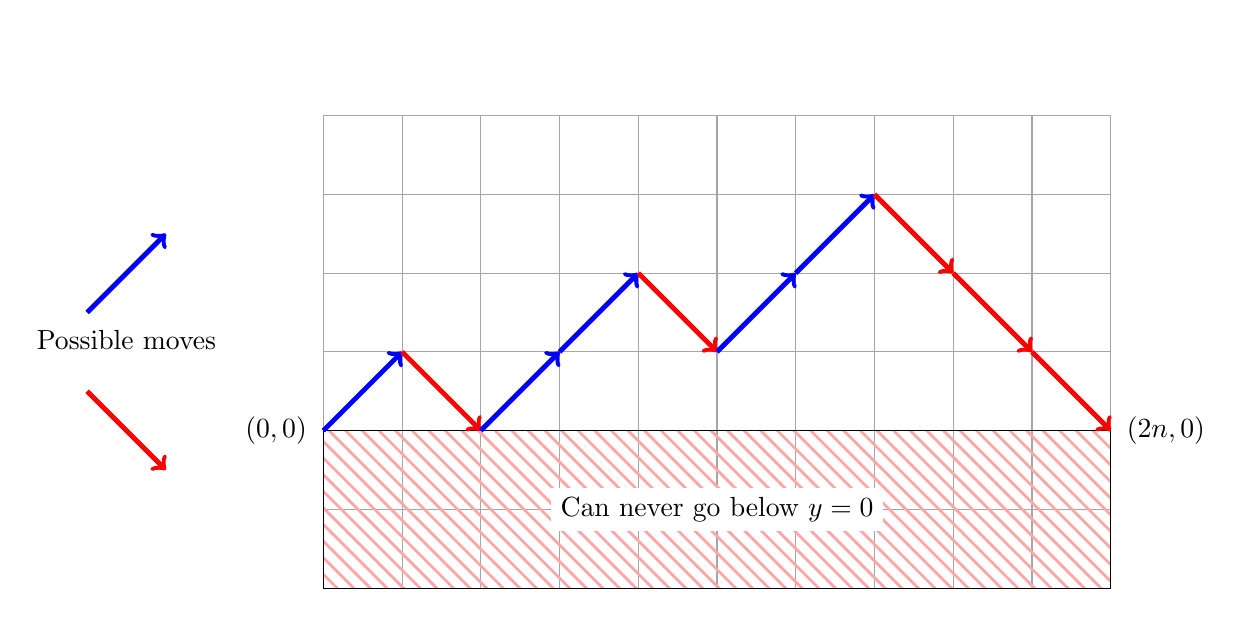
\begin{tikzpicture}
\draw[step=1.0,black,thin,color=black,opacity=.35] (-5,-2) grid (5,4);
\node (S) at (-5, 0) {};
\node (E) at (5, 0) {};
\node (T) at (-5, 5) {};

\draw[pattern=bigger north west lines, pattern color=red!35] (-5,0) rectangle (5,-2) node [midway,fill=white] {Can never go below $y=0$};


\draw [->,line width=1.75,blue] (-8,1.5) -- (-7,2.5) node[midway, black, yshift=-2.4em] {Possible moves};
\draw [->,line width=1.75,red]  (-8,0.5) -- (-7,-.5);

\draw [->,line width=1.75,blue] (-5,0) -- (-4,1);
\draw [->,line width=1.75,red] (-4,1) -- (-3,0);
\draw [->,line width=1.75,blue] (-3,0) -- (-2,1);
\draw [->,line width=1.75,blue] (-2,1) -- (-1,2);
\draw [->,line width=1.75,red] (-1,2) -- (0,1);
\draw [->,line width=1.75,blue] (0,1) -- (1,2);
\draw [->,line width=1.75,blue] (1,2) -- (2,3);
\draw [->,line width=1.75,red] (2,3) -- (3,2);
\draw [->,line width=1.75,red] (3,2) -- (4,1);
\draw [->,line width=1.75,red] (4,1) -- (5,0);
\node [black] at (-5.6,0) {$(0,0)$};
\node [black] at (5.7,0) {$(2n,0)$};
\end{tikzpicture}
\end{center}

$C_n$ is also the number of distinct trees with $n$ nodes (where nodes are read left to right, so for example reflection symmetry doesn't count).
\pagebreak


\section{Principle of Inclusion-Exclusion}
\subsection{General}
The size of the union of $n$ sets $S_1, S_2, \ldots, S_n$ can be computed in terms of intersections of those sets. This is handy when intersections are easier to count than unions.\\

Example for $n=4:$
\newcommand{\dlist}[1]{S_{#1}}
\begin{multline*}
    |\dlist{1} \cup \dlist{2} \cup \dlist{3} \cup \dlist{4}| = |\dlist{1}| + |\dlist{2}| + |\dlist{3}| + |\dlist{4}|\\ 
    -|\dlist{1} \cap \dlist{2}| - |\dlist{1} \cap \dlist{3}| - |\dlist{1} \cap \dlist{4}| - |\dlist{2} \cap \dlist{3}| - |\dlist{2} \cap \dlist{4}| - |\dlist{3} \cap \dlist{4}|\\
    +|\dlist{1} \cap \dlist{2} \cap \dlist{3}| + |\dlist{1} \cap \dlist{2} \cap \dlist{4}| + |\dlist{1} \cap \dlist{3} \cap \dlist{4}| + |\dlist{2} \cap \dlist{3} \cap \dlist{4}|\\
    -|\dlist{1} \cap \dlist{2} \cap \dlist{3} \cap \dlist{4}|
\end{multline*}
\subsection{Derangements}
\[
    D(n) = n!\sum_{i=0}^n \frac{(-1)^i}{i!} = n! - \frac{n!}{1!} + \frac{n!}{2!} - \frac{n!}{3!} +\ldots \approx \frac{n!}{e}
\]

%\[xC^2(x)-C(x) + 1 = 0\]
\pagebreak
\section{Generating Functions}
\subsection{Common Generating Functions}
\begin{equation*}
    \setlength{\jot}{.5cm}
    \begin{aligned}
    \frac{1}{1-x} &= 1 + x + x^2 + x^3 + \ldots & 1, 1, 1, \ldots\\  
    \frac{1-x^{n+1}}{1-x} &= 1 + x + x^2 + x^3 + \ldots x^n & \underbrace{1, 1, 1, \ldots}_{n\text{ ones}}\\
    \frac{1}{1+x} &= 1 - x + x^2 - x^3 + \ldots & 1, -1, 1, -1, \ldots\\  
    \frac{1}{1-x^k} &= 1 + x^k + x^{2k} + x^{3k} + \ldots & 1, \underbrace{0,0,\ldots,0}_{k-1\text{ zeroes}}, 1, 0,\ldots\\
    \frac{1}{1-ax} &= 1 + ax + a^2x^2 + a^3x^3 + \ldots & 1, a, a^2, \ldots\\
    \end{aligned}
\end{equation*}

\subsection{Extended Binomial Theorem}
\begin{equation*}
    \setlength{\jot}{.5cm}
    \begin{aligned}
    \binom{-n}{k} &= (-1)^k\binom{n+k-1}{k}\\
    \binom{n}{k} &= \frac{n(n-1)(n-2)\ldots(n-k+1)}{k!}
    \end{aligned}
\end{equation*}



\section{Probability}


\termtable{
\term{$\Omega$} \emph{Sample Space}, or set of \emph{outcomes}, e.g. coin flip is ${\{H, T\}}$\\
\term{event $E$} Subset of $\Omega$, e.g. $\{H\} \subset \{H, T\}$\\
\term{$E^C$} The \emph{complement} of an event $E \subset \Omega$, or $\Omega\backslash E$\\
\term{event space} The set of events\\
\term{$P:\{0, 1\}^\Omega \rightarrow [0,1]$ } A \emph{probability measure} is a function with domain (subsets of $\Omega$) to a real number in $[0,1]$ subject to the following rules:
    \begin{enumerate}
    \item $P(\emptyset) = 0$ 
    \item $P(\Omega) = 1$
    \item if $A$ and $B$ are disjoint, then $P(A\cup B) = P(A) + P(B)$
    \end{enumerate}\\
\term{$P(A|B)$} The \emph{conditional probability} of $A$ given $B$. \[ P(A|B) =\frac{P(A) \cup P(B)}{P(B)} \] \\
\term{random variable} $X: \Omega \rightarrow T$ (usually $T = \mathbb{R}$)\\
\term{distribution of r.v.} For T arbitrary (but discrete) it's a bar graph\\
\term{$E[X]$} The \emph{expectation} given $(T = \mathbb{R})$ is defined as \[ \sum_{x\in T} x P(X=x)\]\\
\term{uniform distribution} All outcomes have equal probability\\
\term{linearity of expectations} $E[X + Y] = E[X] + E[Y]$ Expected number of heads in three flips is equal to number of heads in flip1, number in flip2, number in flip3, therefore $E[X] = 3E[X_i]$ Does not require independence!\\
\term{Baye's theorem} $P(B|A) = \frac{P(B) P(A|B)}{P(A)}$\\
}

\section{Graphs}

\termtable{
\term{simple graph $G$} Set of vertices $V(G)$ and set of edges $E(G)$\\
\term{$V(G)$} The set of vertices in $G$. Can be any set\\
\term{$E(G)$} The set of edges in $G$. An edge is a set of two \emph{distinct} elements of V(G). $\{v_1, v_2\}: v_1 \neq v_2$\\
\term{directed graph} Same as a simple graph, but edges are length-2 lists, so you can have an edge $(v_1, v_2)$ without the reverse edge $(v_2, v_1)$\\
\term{isomorphism} Two graphs are the same if you rename the vertices. Formally, there exists a bijective function $f: V(G_1) \rightarrow V(G_2)$ such that $\{v, w\} \in E(G_1) \iff \{f(v), f(w)\} \in E(G_2)$ (Note: $\iff$ means \say{if and only if})\\
\term{path} A sequence $v_1 \xrightarrow[e_1]{} v_2 \xrightarrow[e_2]{} v_3 \dots v_k$ where no vertex appears twice\\
\term{cycle} A \emph{path} $v_1 \xrightarrow[e_1]{} v_2 \xrightarrow[e_2]{} v_3 \dots v_1$ which ends at the start vertex\\
\term{tree} A graph with no cycles. There are $n^{n-2}$ trees on $n$ vertices (not expected to prove this)\\
\term{bipartite graph} A graph in which no odd-length cycles exist. The vertices can be divided into disjoint subsets $A$ and $B$ such that no two vertices in $A$ are connected by an edge and no two vertices in $B$ are connected by an edge\\
\term{weighted graph} A graph in which each edge has an number\\
\term{$C_n$} A graph on $n$ vertices where all vertices are in one big cycle\\
\term{$K_n$} A \emph{complete} graph on $n$ vertices (all possible edges exist)\\
\term{$K_{n,m}$} A \emph{bipartite} graph with $n$ vertices in one set and $m$ vertices in the other. Every edge between a vertex in $n$ and a vertex in $m$ exists, and no other edges exist.\\
}
\pagebreak
\section{Groups}
A group $G$ is a \textbf{set} with a function $G\times G \rightarrow G$ such that:
\begin{enumerate}
    \item \emph{Identity}: There exists $\textbf{id} \in G$ such that $\textbf{id}*g = g$ for all $g \in G$.
    \item \emph{Closure}: For all $g_1, g_2 \in G$, $g_1*g_2 \in G$
    \item \emph{Associativity}: $(g_1*g_2)*g_3 = g_1*(g_2*g_3)$
    \item \emph{Inverse}: For all $g$, there exists $g^{-1} \in G$ such that $g*g^{-1} = \textbf{id}$
\end{enumerate}


\termtable{
\term{subgroup} A subgroup $H$ of $(G,*)$ is a subset of G which is a group under *.\\
\term{permutation group} A subgroup of $S_n$\\
\term{cyclic group $C_n$} A subset of $S_n$. (Not the cycle graph $C_n$ or the Catalan number $C_n$)

}
\subsection{Examples}
\begin{itemize}
\item $(\mathbb{R},*)$ is not a group because 0 has no inverse.
\item $(\mathbb{R}\backslash\{0\},*)$ is a group with $\textbf{id} = 1$
\item $(\mathbb{R},+)$ is a group with $\textbf{id} = 0$
\item $(\mathbb{R}\backslash\{0\},*)$ is a group with $\textbf{id} = 1$
\item $(\mathbb{Z}\slash 7\mathbb{Z},+)$ is a group with $\textbf{id} = 1$. $\mathbb{Z}\slash 7\mathbb{Z}$ means using modular arithmetic, so $5 + 5 = 3$ (because 10 mod 7 is 3).
\item $(\mathbb{Z}\slash n\mathbb{Z}\backslash\{0\},*)$ is a group with $\textbf{id} = 1$ if and only if $n$ is prime. If $n$ is composite, then there is then for let $f$ be a factor of $n$. There is no $f^{-1}$ because $f$ times anything is never going to be 1.
 
\end{itemize}

\section{Group Actions}

\termtable{
\term{permutation} A function $g: \{1,2,\dots,n \} \rightarrow \{1,2,\dots,n\} $ which is a bijection. Example: $f(1) = 2, f(2) = 4, f(3) = 3, f(4) = 1$. Can be written $\left(\frac{1234}{2431}\right)$ or $(2431)$\\
\term{$S_n$} The set of all permutations of size $n$. $|S_n| = n!$\\

\term{composition} A composition of permutations $g_1$ and $g_2$ is also a permutation. $g_1(g_2(x))$ is written as $(g_1g_2)(x)$ or $g_1 \circ g_2 (x)$. (Note that you need to apply the permutations from right to left)\\
\term{(id)} The permutation which sends x to itself, e.g. $f(x) = x$\\
\term{associativity} A composition of permutations is associative, meaning $(g_1g_2)g_3 = g_1(g_2g_3)$.\\
\term{inverse} For all $g$, there exists $g^{-1}$ such that $g\circ g^{-1} = \textbf{(id)}$\\
\term{\parbox{4cm}{\raggedleft directed graph notation}} 
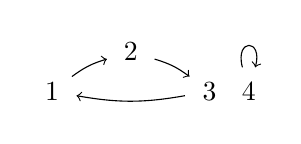
\begin{tikzpicture}
\node[shape=circle] (A) at (0,0) {$1$};
\node[shape=circle] (B) at (1,.5) {$2$};
\node[shape=circle] (C) at (2,0) {$3$};
\node[shape=circle] (D) at (2.5,0) {$4$};
\draw [->] (A) edge[bend left=10] (B);
\draw [->] (B) edge[bend left=10] (C);
\draw [->] (C) edge[bend left=10] (A);
\draw [->] (D) edge[loop above,looseness=6] (D);
\end{tikzpicture}
Every permutation can be represented as a directed graph where each node has one incoming edge and one outgoing edge. Every node participates in exactly one cycle.
\\
\term{cycle notation} Expresses a permutation in terms of cycles. The above example is written $(123)(4)$. This is very handy for performing multiplication. To multiply $A\times B$, for each number find the next number in the $B$-cycle, then find the number after that in the $A$-cycle, and put that in the result. As soon as you get back to the first number in your cycle, start a new cycle. Example: $\Big[(123)(465)\Big] \times \Big[(13542)(6)\Big] = (1)(2)(34)(56)$ (First digit: $1\rightarrow3$ in $B$, then $3\rightarrow1$ in $A$, so 1 is in a cycle by itself in the result)\\
}


\section{Coloring}

\termtable{
\term{coloring} A coloring is a function $f: S \rightarrow C$, where $S$ is a set and $C$ is a set of colors.\\
\term{$\overline{g}$} s\\
}







\end{document}
